\chapter{A Regularized Time Varying Vector Error Correction Model}

In the last chapter, the Online Vector Error Correction Model (OVECM) was
proposed. OVECM parameters are obtained using the Ordinary Least Squares (OLS)
method. Even though OLS is extensively used, it has over-fitting issues and is
computationally expensive. Therefore, OVECM parameters could be very sensitive
to the data. Ridge Regression (RR) is commonly used instead of OLS to tackle
this problem, introducing a regularization parameter which could improve
prediction error. In this chapter, the use of Ridge Regression (RR) and its
variant called Aggregating Algorithm for Regression (AAR) is explored in order
to get better generalisation capability. 

\section{The problem}

VECM model parameters are traditionally obtained using ordinary least squares
(OLS) method. OLS has two main problems: is sensitive to input data errors
and involves many calculations. The former problem is commonly solved using
Ridge Regression (RR) \cite{hoerl1970} which introduces a regularization
parameter that leads to an unbiased estimation with better generalization
capability. The second problem of computational complexity depends on the number
of past values and observations considered.  Recently, online learning
algorithms have been proposed to solve problems with large data sets because of
their simplicity and their ability to update the model when new data is
available. 

The proposal is to create an online algorithm based on the idea of OVECM
using either RR or its variant AAR instead of OLS 
. 


\section{Methodology}

OVECM only considers a time varying window of historical data and uses OLS to
get solve model parameters. This proposal is about using RR or its variant AAR
as an alternative of OLS to get model parameters.

Since cointegration vectors represent a long-run relationship between the time
series, they vary little in time. This proposal also includes to obtain new
cointegration vectors only when this long-term relationship changes. This change
is detected by tracking the Mean Absolute Percentage Error (MAPE) of the last
$n$ in-sample forecasts.


VECM($p$) matrix form is:

\begin{equation}\label{eq:vareq}
\mathbf{B} = 
\mathbf{A} \mathbf{X} + 
\mathbf{E} \, , 
\end{equation}

\noindent where matrix $\mathbf{B},\mathbf{X},\mathbf{E}$ and $\mathbf{A}$ were
previously defined in equations \ref{eq:vecY} , \ref{eq:vecX} , \ref{eq:vecE} and
\ref{eq:vecA} respectively.

In the traditional VECM the number of rows of matrix $\mathbf{A}$ increases with the number of
observations $\mathbf{y}_t$. This proposal considers only the most recent $L$
rows of matrices $\mathbf{A}$ and $\mathbf{B}$ defined as  $\mathbf{A}(t)$ and
$\mathbf{B}(t)$:

\begin{equation}
\label{eq:notation}
	\mathbf{A}(t) = 
\left[
  \begin{tabular}{c>{$}c<{$}c}
    --- & \mathbf{a}^{\top}_{t-L} & ---\\
    --- & \mathbf{a}^{\top}_{t-L+1} & ---\\
    & \vdots & \\
    --- & \mathbf{a}^{\top}_{t} & ---
  \end{tabular}
\right]
\quad \text{and} \quad
\mathbf{B}(t) =
\left[
  \begin{tabular}{c>{$}c<{$}c}
    --- & \mathbf{b}_{t-L} & ---\\
    --- & \mathbf{b}_{t-L+1} & ---\\
    & \vdots & \\
    --- & \mathbf{b}_{t} & ---
  \end{tabular}
\right] \, ,
\
\end{equation}

\noindent so that VECM parameters $\mathbf{X}(t)$ are found using the following
equation:

\begin{equation}
\mathbf{B}(t) = \mathbf{A}(t) \mathbf{X}(t) + \mathbf{E}(t)\\
\end{equation}

The RR solution $\mathbf{\hat{X}}(t)$ using the sliding window matrices defined above
is:

\begin{equation}
\label{eq:oproblem}
\mathbf{\hat{X}}(t)=\mathbf{S}(t)^{-1} \mathbf{W}(t) \, ,
\end{equation}

\noindent where $\mathbf{S}{t}$ and $\mathbf{W}{t}$ are define as:

\begin{eqnarray*}
\mathbf{S}(t) =&{\bf A}(t)^\top{\bf A}(t)+ \lambda \mathbb{I} &=
\sum_{i=0}^L \mathbf{a}_{t-i}\mathbf{a}_{t-i}^\top + \lambda \mathbb{I}
\label{eq:S} \\
\mathbf{W}(t) =& {\bf A}(t)^\top{\bf B}(t) &= 
\sum_{i=0}^L \mathbf{a}_{t-i}\mathbf{b}_{t-i} 
\label{eq:W}
\end{eqnarray*}

It is worth noticing that, at the next time step, the matrices $\mathbf{S}(t+1)$
and $\mathbf{W}(t+1)$ are slightly different to $\mathbf{S}(t)$ and
$\mathbf{W}(t)$:

\begin{eqnarray*}
\mathbf{S}(t+1)&=&
\mathbf{S}(t) +
\mathbf{a}_{t+1}
\mathbf{a}_{t+1}^\top -
\mathbf{a}_{t-L} \mathbf{a}_{t-L}^\top \\
\mathbf{W}(t+1)&=&
\mathbf{W}(t) +
\mathbf{a}_{t+1}
\mathbf{b}_{t+1} -
\mathbf{a}_{t-L} \mathbf{b}_{t-L} \, .
\end{eqnarray*}

%Agregar solo si se decide agregar Sherman-Morrison
%Therefore the Sherman-Morrison-Woodbury formula can be used to reduce inverse matrix
%calculations.

The algorithm~\ref{alg:proposal} shows OVECM using three different
methods for geting model parameters: OLS, RR, AAR which leads to three different
algorithms OVECM-OLS, OVECM-RR, OVECM-AAR:

\begin{algorithm}[ht]
\begin{algorithmic}[1]
\REQUIRE $\,$ \\
$\mathbf{y}$: matrix with $N$ input vectors and $l$ time series\\
$p$: number of past values \\
method: \{'OLS','RR','AAR'\} \\
$\lambda$: regularization parameter (only requires for RR and AAR methods) \\
$L$: window size of data($L<N$) \\
$\text{mean\_error}$: MAPE threshold \\
$n$: windows size to obtain in-sample MAPE \\
\ENSURE  $\,$ \\
$\{\mathbf{y}_{\text{pred}}[L+1],\dots, \mathbf{y}_{\text{pred}}[N]\}$: model predictions 
\STATE solver = new \texttt{Solver}(method,$\lambda$) \\
\FOR { $t =1$ to $N-L$ }
    \STATE $\mathbf{Y} \gets \mathbf{y}[t:t+L-1]$
    \STATE $\mathbf{y}_t \gets \mathbf{y}[t+L]$
	\IF {$t = 1$}
	    \STATE{$v \gets \texttt{getJohansen}(\mathbf{Y},p)$}
	    \STATE{$[\mathbf{A} \quad \mathbf{B}] \gets
        \texttt{vecMatrix}(\mathbf{Y},p,v)$}
        \STATE \texttt{solver.init\_model($\mathbf{A},\mathbf{B}$)} 
    \ENDIF
	\STATE{[$\mathbf{A} \quad \mathbf{B} \quad \mathbf{a}_t \quad \mathbf{a}_L \quad \mathbf{b}_t \quad
    \mathbf{b}_L ] \gets
    \texttt{vecMatrixOnline}(\mathbf{Y},\mathbf{y}_t,p,v)$}
    \STATE $[\mathbf{X} \quad \mathbf{y}_{\text{pred}}[t]] \gets \texttt{solver.regression}
    (\mathbf{A},\mathbf{B},\mathbf{a}_t,\mathbf{b}_t)$
    \STATE $\mathbf{Y}_{\text{pred}} = \mathbf{AX}[-n:]+\mathbf{Y}[-n-1:-1]$
    \STATE $\mathbf{e} = \texttt{mape}(\mathbf{Y}_{\text{pred}},\mathbf{Y}[-n:])$
    \IF {$\texttt{mean}(\mathbf{e}) > \text{mean\_error}$}
	    \STATE{$v \gets \texttt{getJohansen}(\mathbf{Y},p)$}
	    \STATE{$\mathbf{A} \gets
        \texttt{vecMatrixUpdate}(\mathbf{A},\mathbf{Y},p,v)$}
        \STATE \texttt{solver.init\_model($\mathbf{A},\mathbf{B}$)} 
	    \STATE{$[\mathbf{a}_t \quad \mathbf{b}_t] \gets
        \texttt{vecMatrixOnline}(\mathbf{Y},\mathbf{y}_t,p,v)$}
        \STATE $[\mathbf{X} \quad \mathbf{y}_{\text{pred}}[t]] \gets \texttt{solver.regression}
        (\mathbf{A},\mathbf{B},\mathbf{a}_t,\mathbf{b}_t)$
    \ENDIF
\STATE{$[\mathbf{A} \quad \mathbf{B}] \gets
\texttt{matrixUpdate}(\mathbf{A},\mathbf{B},\mathbf{a}_t,\mathbf{b}t)$}
\ENDFOR
\end{algorithmic}
\caption{OVECM: Online VECM}
\label{alg:proposal}
\end{algorithm}

The proposal considers the following:

\begin{itemize}
\item The function \texttt{getJohansen} returns cointegration vectors given by the
Johansen method considering the trace statistic test at 95\% level of
significance. This procedure is called at the first step of the algorithm and
every time in-sample MAPE ($\mathbf{e}$) exceeds threshold error defined (mean\_error).
\item The function \texttt{vecMatrix} returns VECM
matrices $\mathbf{A}(t),\mathbf{B}(t)$ shown in equation~(\ref{eq:notation}). This
method is only required at the first step.
\item The function \texttt{vecMatrixOnline} returns new rows $\mathbf{a}_t^\top$ and
$\mathbf{b}_t^\top$ given new input data $\mathbf{y}_t$.
\item The Solver class (see algorithm \ref{alg:solver}) obtain VECM parameters  
using RR, AAR or OLS methods.
\item The function \texttt{vecMatrixUpdate} updates matrix $\mathbf{A}$ when new
cointegration vectors are required (matrix $\mathbf{B}$ is not affected). Model
parameters $\mathbf{X}$ is also updated later.
%\item The number of cointegration vectors is set as a parameter (aun no lo
%coloco en el algoritmo).
%\item In order to set VECM parameter: $L$ and $p$, we use the Akaike Information
%Criterion (AIC). RR parameter $\lambda$ was done by cross-validation.
%\item Obtain VECM parameter $\mathbf{X}(t)$ in equation \ref{eq:optsolSLAAR} requires
%to calculate the inverse of matrix $\mathbf{S}(t+1)$ which is an expensive
%routine.However, since we already know $\mathbf{S}(t)^{-1}$ we can use
%Sherman-Morrison-Woodbury twice~\ref{eq:SMW}.
\end{itemize}




\begin{algorithm}[ht]
\begin{algorithmic}[1]
\REQUIRE $\,$ \\
method: \{'OLS','RR','AAR'\} \\
$\mathbf{A}$: VECM design matrix \\
$\mathbf{B}$: VECM dependant variables \\
$\mathbf{a}_t$: new row of $\mathbf{A}$ \\
$\mathbf{b}_t$: new row of $\mathbf{B}$ \\
$\gamma$: regularization parameter \\
$n$: windows size to obtain in-sample MAPE \\
\ENSURE  $\,$ \\
$\mathbf{X}$: regression solution \\
$\mathbf{e}$: in-sample MAPE \\
%\quad \\
%\texttt{init}($L,\lambda$)
%\STATE self.L = L
%\STATE self.lambda = $\lambda$
\quad \\
\texttt{init\_model}($\mathbf{A},\mathbf{B}$)
\STATE $ [m \quad n] = \text{size}(\mathbf{A}) $ 
\STATE $\mathbf{S} = \displaystyle \sum_{i=1}^m \mathbf{a}_i \mathbf{a}_i^\top + \gamma \mathbb{I}$
\STATE $\mathbf{W} = \displaystyle \sum_{i=1}^m \mathbf{a}_i \mathbf{b}_i$
\quad \\
\texttt{regression}($\mathbf{A},\mathbf{B},\mathbf{a_t},\mathbf{b_t}$) \\
\IF {method == 'OLS'}
        \STATE $\mathbf{X}=(\mathbf{A}^\top \mathbf{A})^{-1}\mathbf{A}^\top
        \mathbf{B}$
\ELSIF {method == 'RR'}
        \STATE $\mathbf{X} = \mathbf{S}^{-1} \mathbf{W} $
        \STATE $\mathbf{S} = \mathbf{S}+
        \mathbf{a}_t \mathbf{a}_t^\top-
        \mathbf{a}_1 \mathbf{a}_1^\top$
        \STATE $\mathbf{W} = \mathbf{W} + \mathbf{a}_t \mathbf{b}_t$
\ELSIF {method == 'ARR'}
        \STATE $\mathbf{S} = \mathbf{S}+
        \mathbf{a}_t \mathbf{a}_t^\top-
        \mathbf{a}_1 \mathbf{a}_1^\top$
        \STATE $\mathbf{X} = \mathbf{S}^{-1} \mathbf{W} $
        \STATE $\mathbf{W} = \mathbf{W} + \mathbf{a}_t \mathbf{b}_t$
\ENDIF
\STATE $\mathbf{y}_{\text{pred}} = \mathbf{X}^\top \mathbf{a}_t$
\end{algorithmic}
\caption{Solver Class for Regression Methods}
\label{alg:solver}
\end{algorithm}




% Aqui se puede hablar de evaluation using competitive analysis. The idea
%of competitiveness is to compare the output generated by an online algorithm to
%the output produced by an optimal offline algorithm. An optimal online algorithm
%is an omniscient algorithm that knows the entire input data in advance and can
%compute an optimal output. The better an online algorithm approximates the
%optimal solution, the more competitive this algorithm is.


The proposal was compared against an optimal online algorithm which is a time varying
VECM (OOVECM). Algorithm ~\ref{alg:OOVECM} shows this modification:


\begin{algorithm}[ht]
\begin{algorithmic}[1]
\REQUIRE $\,$ \\
$\mathbf{y}$: matrix with $N$ input vectors and $l$ time series\\
$p$: number of past values \\
$L$: sliding window size ($L<N$) \\
\ENSURE  $\,$ \\
$\{\Delta \mathbf{y}_{\text{pred}}[L+1],\dots,\Delta \mathbf{y}_{\text{pred}}[N]\}$: model predictions 
\FOR { $i =0$ to $N-L$ }
    \STATE $\mathbf{y}_i \gets \mathbf{y}[i:i+L]$
	\STATE{$v \gets \texttt{getJohansen}(\mathbf{y}_i,p)$}
	\STATE{$[\mathbf{A} \quad \mathbf{B}] \gets
    \texttt{vecMatrix}(\mathbf{y}_i,p,v)$}
    \STATE $\mathbf{X} \gets \text{OLS} (\mathbf{A},\mathbf{B})$%\mathbf{(A^\top A)^{-1}A^\top B}$
    \STATE $\Delta \mathbf{Y}_{\text{true}}[i] \gets \mathbf{B}[-1,:]$
    \STATE $\Delta \mathbf{Y}_{\text{pred}}[i] \gets \mathbf{A}[-1,:] \times \mathbf{X}$
\ENDFOR
    \STATE $\text{MAPE} \gets \texttt{mape}(\Delta \mathbf{Y}_{\text{true}}, \Delta
    \mathbf{Y}_{\text{pred}})$
\end{algorithmic}
\caption{OOVECM: Optimal Online Vector Error Correction Model}
\label{alg:OOVECM}
\end{algorithm}


%%Solo para tesis
%\section{Online VEC model}
%
%If we want to update the VEC model with new input data
%$\mathbf{y}_{T+1}$, we have to add a new row in matrices
%$\mathbf{Y,X}$ and $\mathbf{E}$. 
%
%\begin{eqnarray}
%\mathbf{Y} &=& 
%                \left[ \begin{array}{ccc}
%               \quad & \mathbf{\Delta y}_{p+1} & \quad \\ \hline
%               \quad & \mathbf{\Delta y}_{p+2} & \quad \\ \hline
%               \quad & \vdots & \quad \\ \hline 
%               \quad & \mathbf{\Delta y}_T & \quad \\ 
%               \quad & \color{red}\mathbf{\Delta y}_{T+1} & \quad 
%               \end{array} \right]
%             \\
%\mathbf{\Phi^*} &=& 
%                \left[ \begin{array}{ccc}
%               \phi_{p-1}^* \\ 
%               \vdots \\ 
%               \phi_{1}^* \\
%               \alpha \\
%                c   
%               \end{array} \right]
%\\
%\mathbf{X} &=& \begin{bmatrix} \label{offX}
%   \mathbf{\Delta y}_2 & \dots & \mathbf{\Delta y}_{p-1} &
%   \mathbf{\Delta y}_{p} & \beta'\mathbf{y}_{p} & 1\\
%   \mathbf{\Delta y}_3 & \dots & \mathbf{\Delta y}_{p} &
%   \mathbf{\Delta y}_{p+1} & \beta'\mathbf{y}_{p+1} &1\\
%   \vdots &  \ddots & \vdots & \vdots & \vdots & \vdots\\
%   \mathbf{\Delta y}_{T-p+1} & \dots & \mathbf{\Delta y}_{T-2} &
%   \mathbf{\Delta y}_{T-1} & \beta'\mathbf{y}_{T-1} &1 \\
%   \color{red} \mathbf{\Delta y}_{T-p+2} & \dots & \color{red}\mathbf{\Delta y}_{T-1} &
%   \color{red}\mathbf{\Delta y}_{T} & \color{red}\beta'\mathbf{y}_{T}
%   & \color{red} 1
%   \end{bmatrix}
%\\
%\mathbf{E} &=& \begin{bmatrix}
%              \mathbf{\epsilon}_{p+1} \\ \vdots \\ \mathbf{\epsilon}_T
%              \\ \color{red}\mathbf{\epsilon}_{T+1}
%             \end{bmatrix}
%\end{eqnarray}



\section{Experiments}

\begin{figure}[!h]
  %\vspace{-0.8cm}
  \centering
  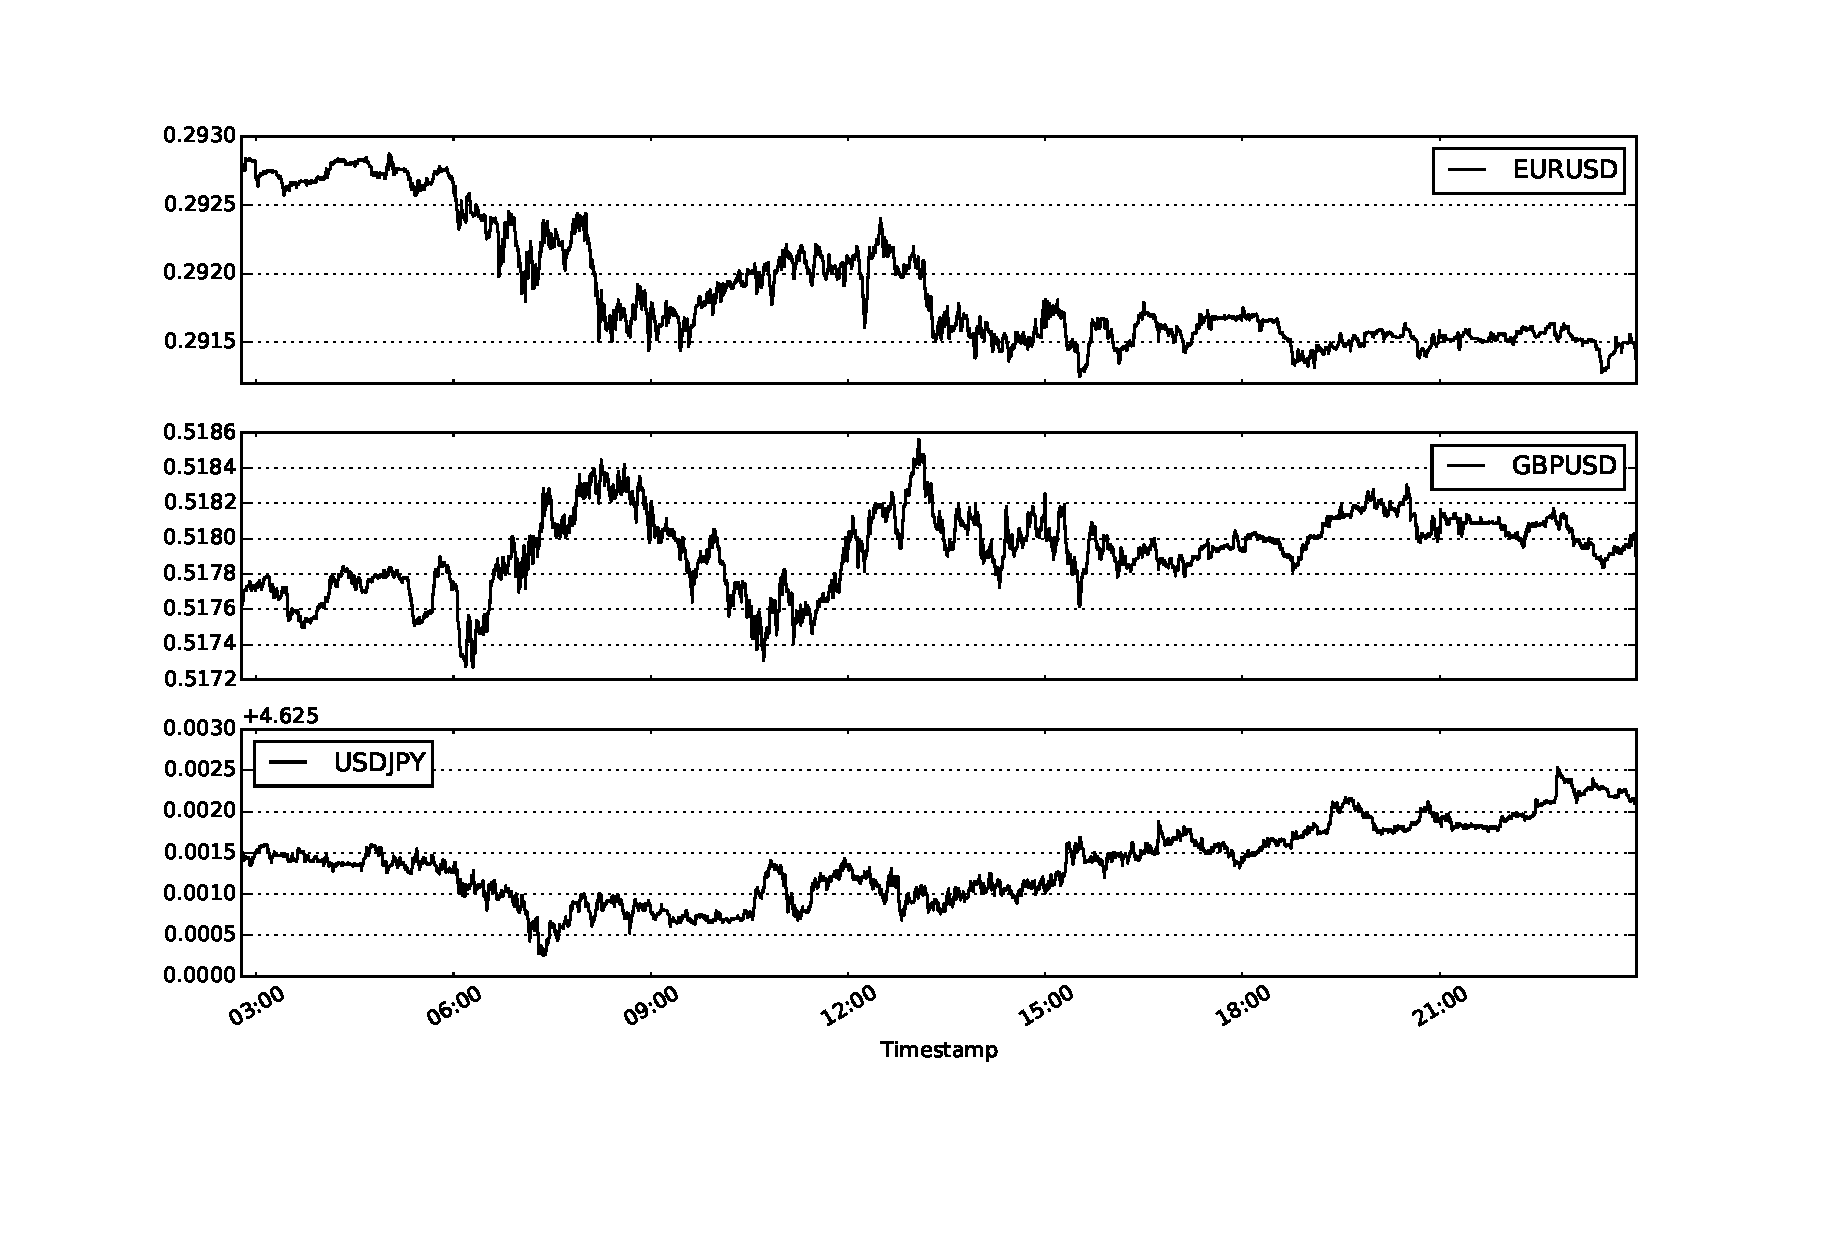
\includegraphics[width=\textwidth]{img/forexdata}
  \caption{10 seconds frequency forex data for EURUSD, GBPUSD and USDJPY}
  \label{fig:forexdata}
\end{figure}

\begin{figure}[!h]
  %\vspace{-0.8cm}
  \centering
  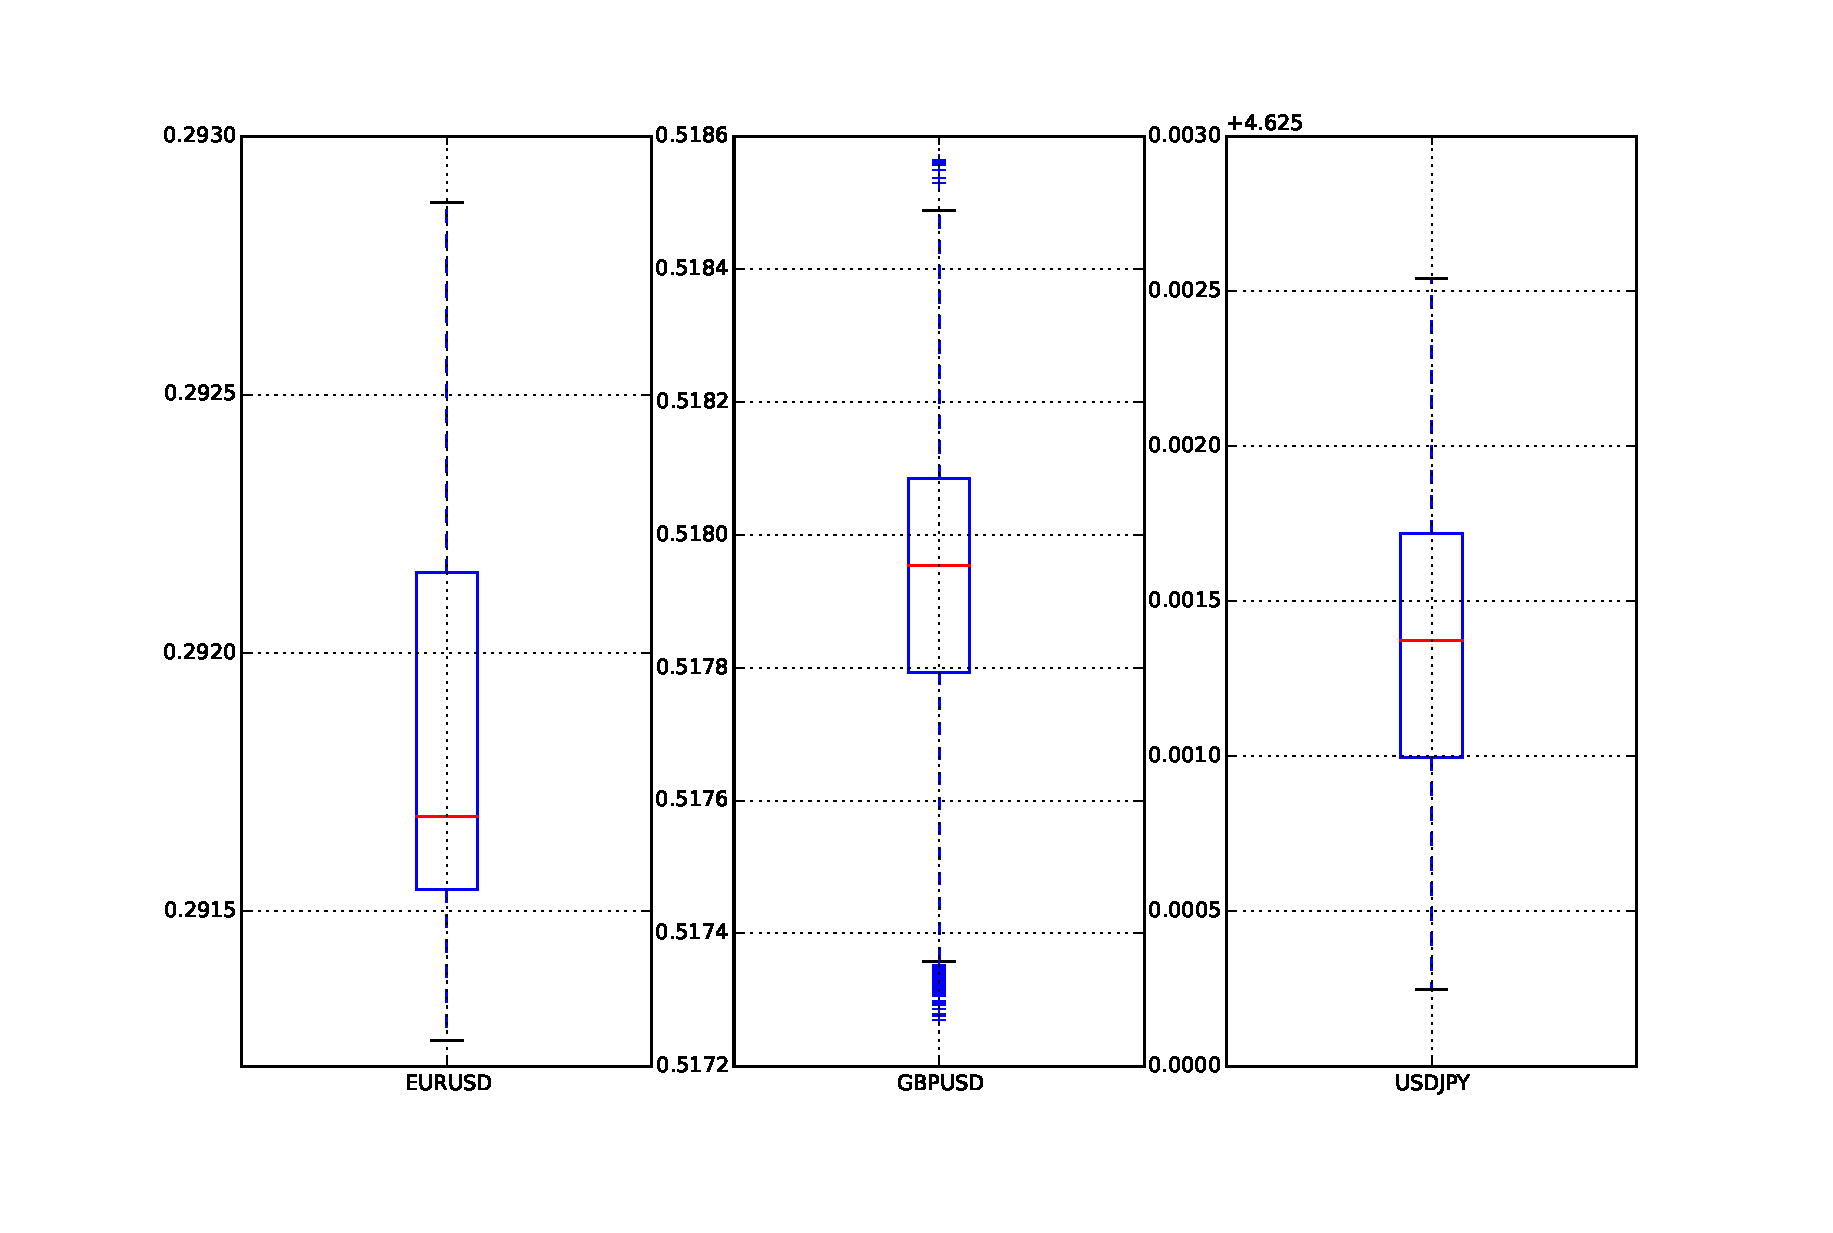
\includegraphics[width=0.8\textwidth]{img/distdata}
  \caption{Distribution of EURUSD, GBPUSD and USDJPY data}
  \label{fig:distdata}
\end{figure}


\begin{figure}[!h]
  %\vspace{-0.8cm}
  \centering
  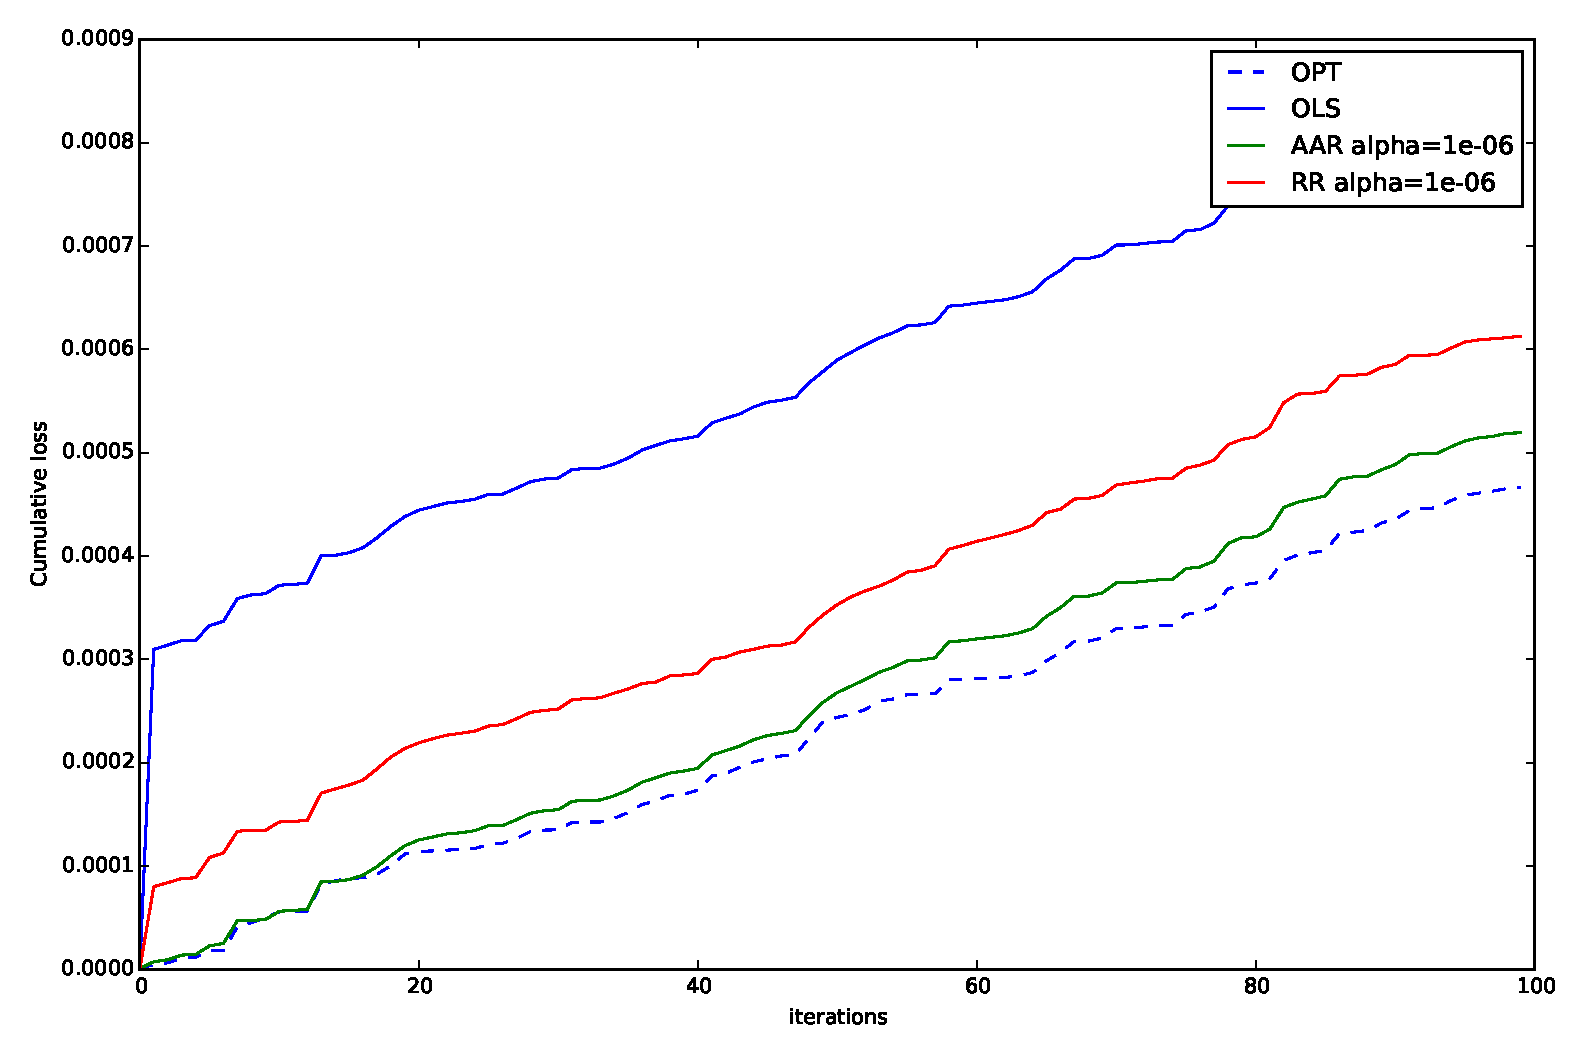
\includegraphics[width=0.9\textwidth]{img/onlinecomparison}
  \caption{Cumulative loss of AAR, RR and OLS solutions for VECM against its optimal algorithm}
  \label{fig:onlinecomparison}
\end{figure}


\begin{figure}[!h]
  %\vspace{-0.8cm}
  \centering
  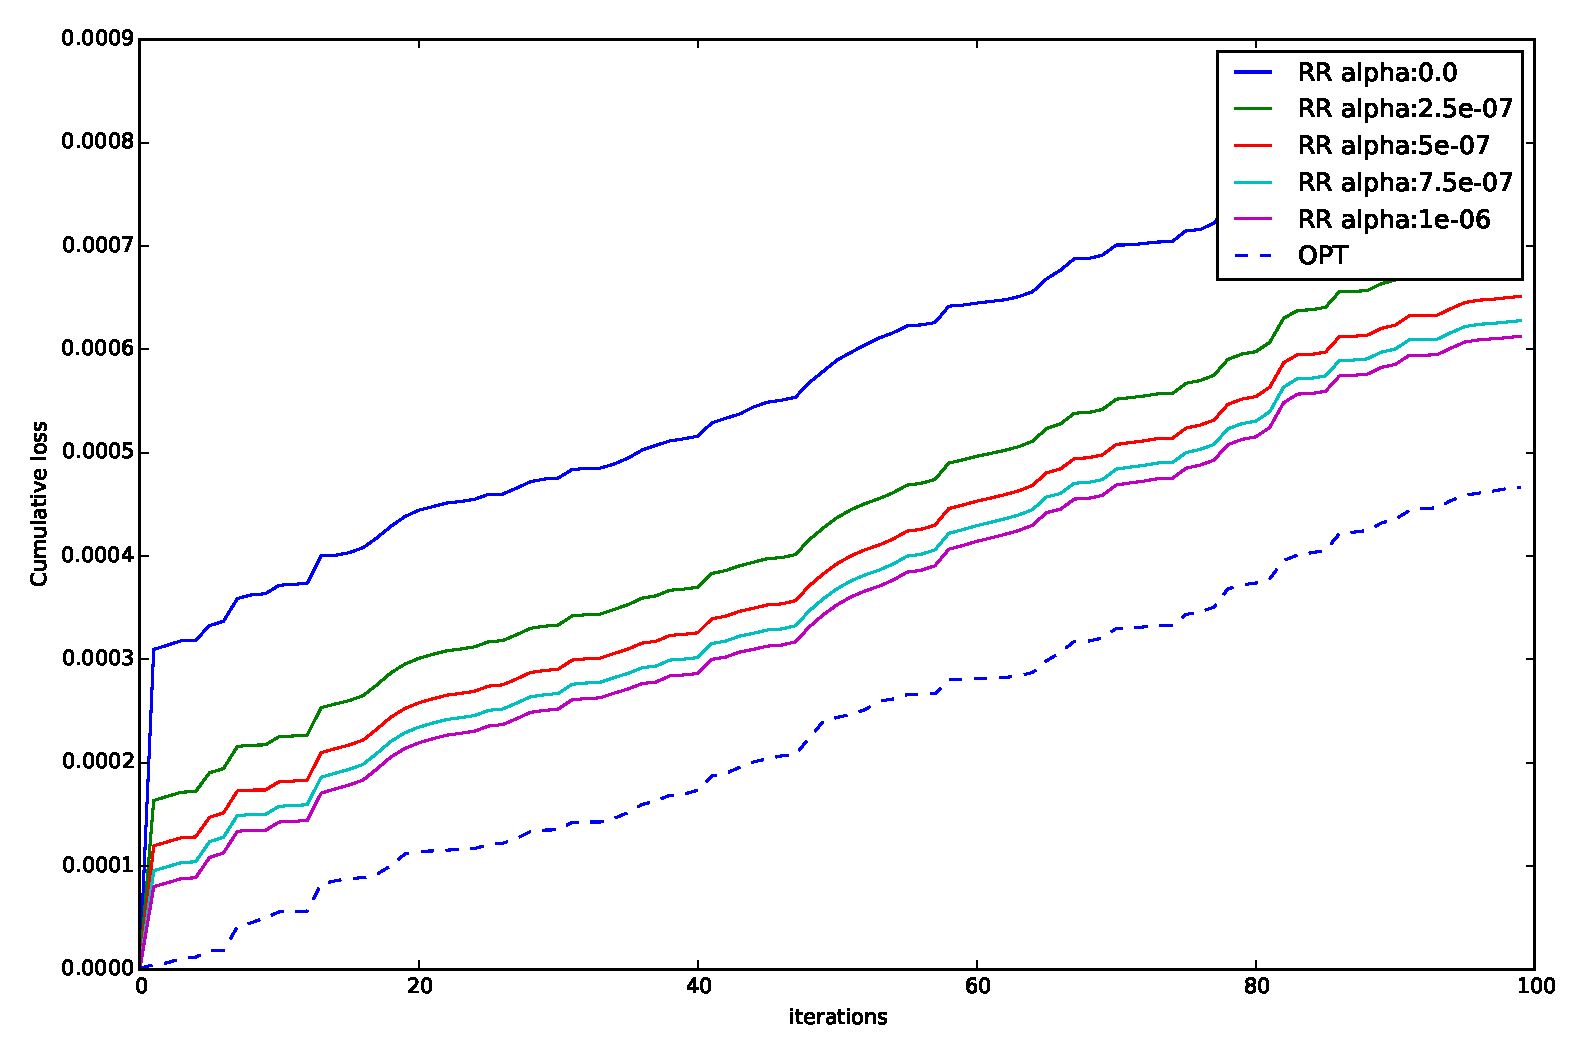
\includegraphics[width=0.9\textwidth]{img/RRcomparison}
  \caption{Cumulative loss RR VECM against its optimal algorithm using different $\lambda$ values}
  \label{fig:RRcomparison}
\end{figure}


\begin{figure}[!h]
  %\vspace{-0.8cm}
  \centering
  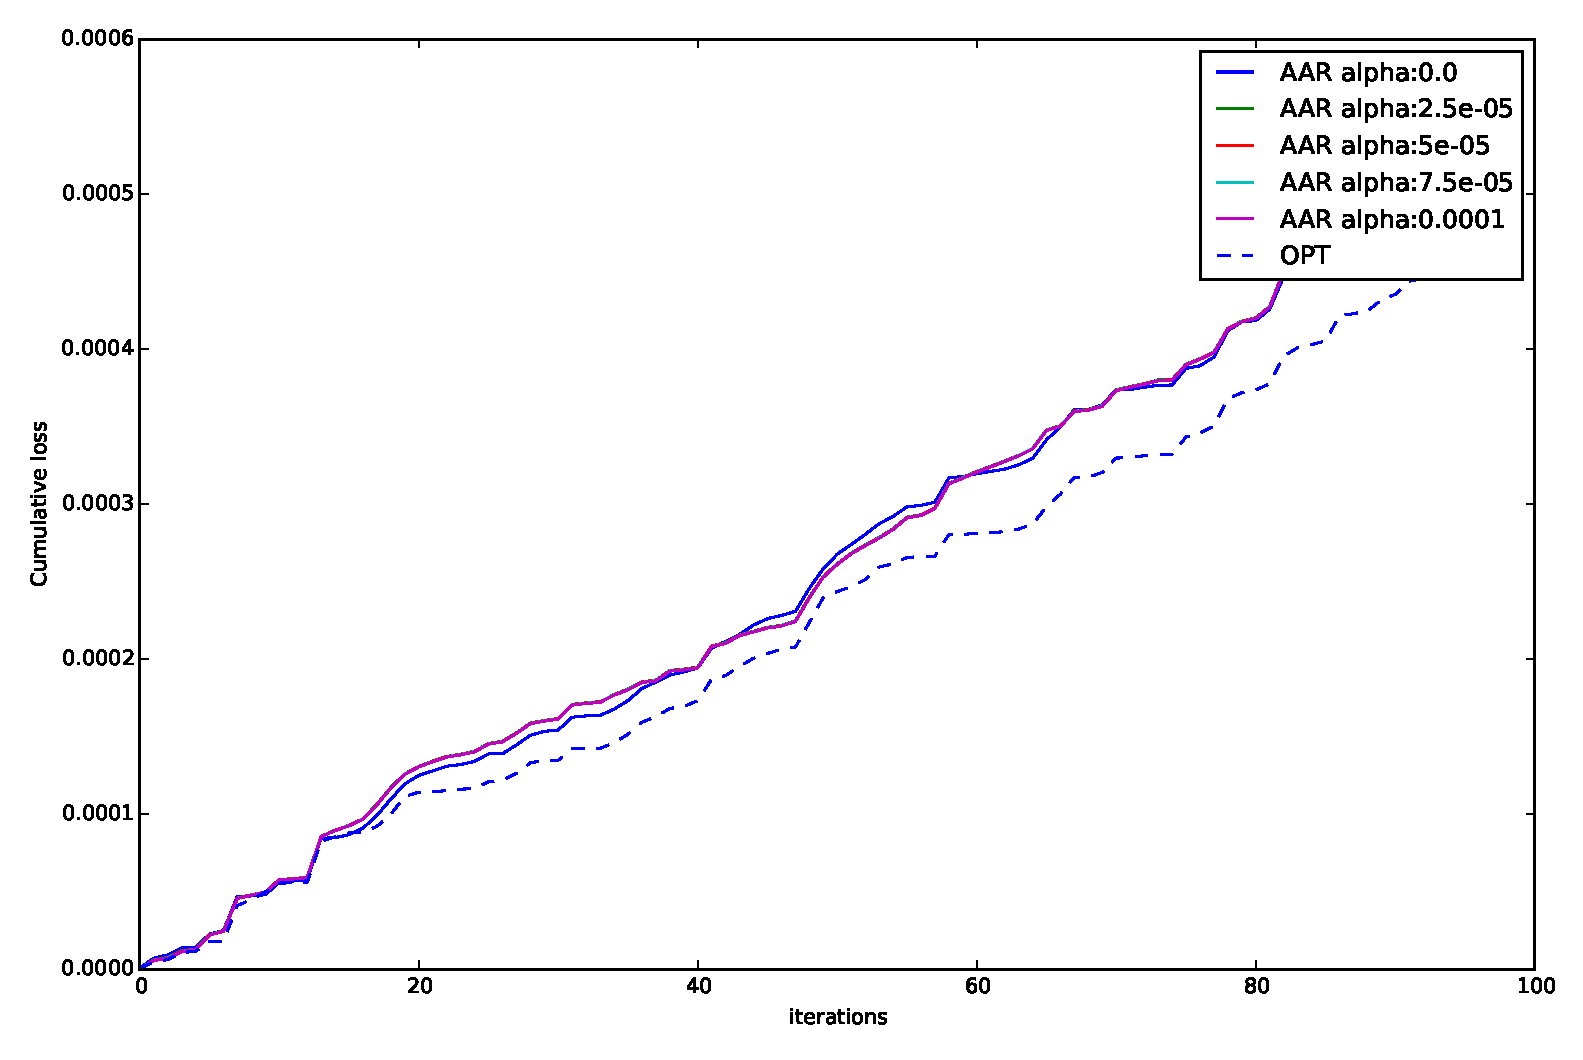
\includegraphics[width=0.9\textwidth]{img/AARcomparison}
  \caption{Cumulative loss AAR VECM against its optimal algorithm using different $\lambda$ values}
  \label{fig:AARcomparison}
\end{figure}

